% ****** Start of file apssamp.tex ******
%
%   This file is part of the APS files in the REVTeX 4.1 distribution.
%   Version 4.1r of REVTeX, August 2010
%
%   Copyright (c) 2009, 2010 The American Physical Society.
%
%   See the REVTeX 4 README file for restrictions and more information.
%
% TeX'ing this file requires that you have AMS-LaTeX 2.0 installed
% as well as the rest of the prerequisites for REVTeX 4.1
%
% See the REVTeX 4 README file
% It also requires running BibTeX. The commands are as follows:
%
%  1)  latex apssamp.tex
%  2)  bibtex apssamp
%  3)  latex apssamp.tex
%  4)  latex apssamp.tex
%
\documentclass[
reprint,
 amsmath,amssymb,
 aps,
 prl
]{revtex4-1}

\newcommand{\partDeriv}[2]{\frac{\partial #1}{\partial #2}}
\DeclareMathOperator\erf{erf}

\usepackage{graphicx}% Include figure files
\usepackage{dcolumn}% Align table columns on decimal point
\usepackage{bm}% bold math
\usepackage{hyperref}


\begin{document}

\title{On The Diffusion of Sticky Particles in 1-D}

\author{Joshua DM Hellier}
 \email{J.D.M.Hellier@sms.ed.ac.uk}
\author{Graeme J Ackland}
 \email{G.J.Ackland@ed.ac.uk}
\affiliation{
 SUPA, School of Physics and Astronomy, University of Edinburgh, Mayfield Road, Edinburgh EH9 3JZ, United Kingdom
}

\date{\today}% It is always \today, today,
             %  but any date may be explicitly specified

\begin{abstract}
The 1D Ising model is the simplest Hamiltonian-based model in
statistical mechanics. The simplest interacting particle process is
the Symmetric Exclusion Process (SEP), a 1D lattice gas of particles
that hop symmetrically and cannot overlap.  Combining the two gives a
model for sticky particle diffusion, SPM, which is described here.
SPM dynamics are based on SEP with short-range interaction, allowing
flow due to non-equilibrium boundary conditions.  We prove that SPM is
also a detailed-balance respecting, particle-conserving, Monte Carlo
description of the Ising model.  Neither the Ising model nor SEP have
a phase transition in 1D, but the SPM exhibits a non-equilibrium
transition.  This is from normal diffusion to a state with close to
zero flow, breaking into a two-phase mixture.  We present a fully
non-linear, analytic, mean-field solution, which has a crossover from
a positive to a negative diffusion constant coincident with the full SPM 
transition. Thus the mean field theory successfully predicts its own demise.
The simplicity of the model suggests a wide range of possible
applications.


\end{abstract}

%\keywords{Suggested keywords}%Use showkeys class option if keyword
                              %display desired
\maketitle




Lattice gases are a ubiquitous tool for modeling complex systems from
biology to traffic~\cite{1742-5468-2011-07-P07007, Mobilia2007,
  tegner2015high, zhu2012atomic, DealGrove1965, MottCabrera1949,
  Buzzaccaro2007}.  Analytically solvable cases involve
non-interacting or excluding particles, but in any real system of
interest the moving objects interact. Many models tackle the situation
where the diffusing objects interact with an external field of the
substrate~\cite{ladd1988application, liggett1985interacting,
  BenNaim1999, Shandarin1989, Frachebourg1999, Frachebourg2000}, and
non-trivial flow is induced by these non-equilibrium interactions.  

For many applications, one is interested in a system where the only
non-equilibrium feature is a driving force applied at the boundaries,
such as a chemical potential difference, while away from the
boundaries the system is free to self-organise.  There is surprisingly
little work considering how complex flow arises only interactions
between the moving particles themselves, allowing the system to
self-organise according to some equilibrium.  One reason for this is
that the interactions introduce nonlinearities in analytical models,
which makes them challenging to solve, at least outside of limits in
which they can be linearized. This is unfortunate because it is
precisely these nonlinearities which introduce interesting behaviors
such as discontinuities at the oxide-metal interface or diffusion
instability~\cite{Obukhovsky2017,Gorokhova2010}.

Here we investigate a simple one-dimensional model, the ``Sticky
Particle Model'' or SPM, specified in the top left inset of
Fig.~\ref{fig:lambdaScans}, which contains such interparticle
interactions.  We explore the impact this has on particle-flow, in
particular when observed in the large-scale limit.

There are many examples of models of driven-dissipative dynamics, it
is sometimes assumed that locally non-equilibrium dynamics are
required to model complex flows. The novel feature of SPM is that it
has locally equilibrium dynamics (i.e. obeys detailed balance) but
still exhibits a nonequilibrium phase transformation from a
homogeneous, diffusing phase to a jammed structure.  It demonstrates that while local
dissipation or substrate interactions can cause non-diffusive flow,
they are not a necessary requirement.


One might contrast this
approach (making a simple microscopic model and trying to learn from
it about large-scale interface growth) with approaches such as the KPZ
equation~\cite{PhysRevLett.56.889, PhysRevA.38.4271, Sasamoto2010}
(where one analyses the extreme large-scale dynamics using
universality classes).

\iffalse
\begin{figure}
\vspace{1em}
    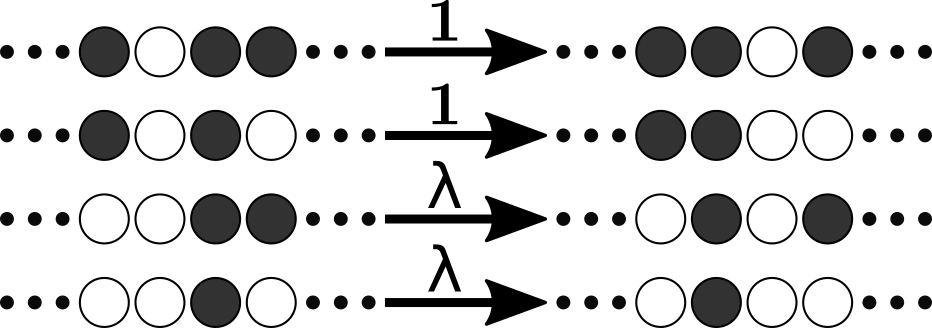
\includegraphics[width=\linewidth]{newRates}
\caption{\label{fig:rates} White circles indicate particles, dark circles indicate empty sites (vacancies). Particles randomly move into adjacent vacancies with rate $1$ (having rescaled time for notational convenience), unless there is a
particle behind the position they're moving from, in which case they move with rate $\lambda$; the state of the site next to the position the particle is moving into is irrelevant.
Particles also move to the left, with rates such that the whole model is totally symmetric.}
    \vspace{-3em}
\end{figure}
\fi

\begin{figure}[h!]
\setbox1=\hbox{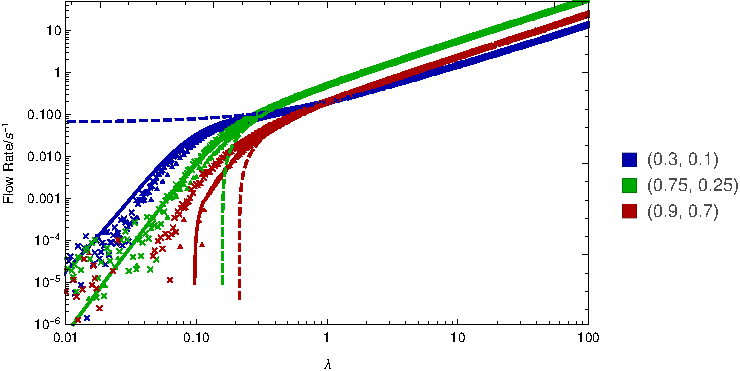
\includegraphics[width=\linewidth]{logFlowRates}}
  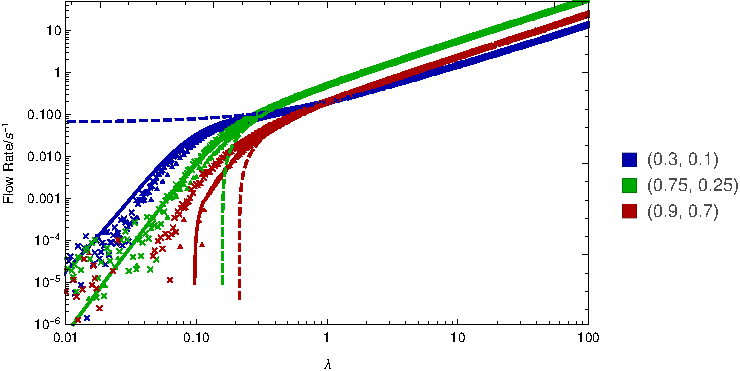
\includegraphics[width=\linewidth]{logFlowRates}\llap{\makebox[0.525\linewidth][l]{\raisebox{0.6cm}{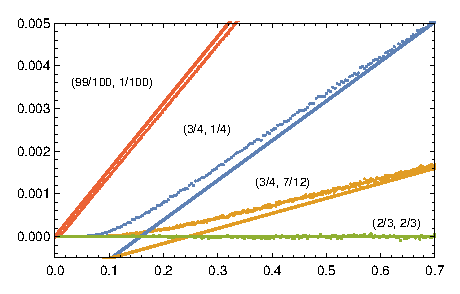
\includegraphics[width=0.475\linewidth]{linearFlowRates}}}}\llap{\makebox[0.9\linewidth][l]{\raisebox{3.75cm}{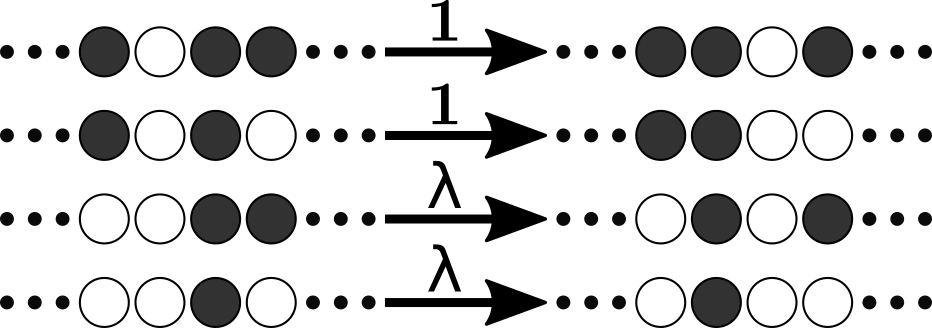
\includegraphics[width=0.45\linewidth]{newRates}}}}
    \vspace{-1em}
\vspace{1em}
\caption{\label{fig:lambdaScans} \textbf{Top left:}  SPM
  dynamics: White circles indicate particles, dark circles indicate
  empty sites (vacancies). Particles randomly move into adjacent
  vacancies with rate $1$,
unless there is an adjacent particle, in which case they move with
rate $\lambda$; the state of the site beyond the new position is
irrelevant.  Particles can move left or right, such that the whole
model is totally symmetric.\\ \textbf{Bottom right:} Mean flow rate
observed as a function of $\lambda$ with fixed boundary densities
$(\rho_0, \rho_L)$ as labeled in the plot.  The MFT predictions are
indicated by the solid line.  Each data point is derive from systems of length
$64$ (length $32$, $128$ and $256$ give similar results), run
for $400000$ Gillespie steps for equilibration followed by $10000$
measurement runs of $1000$ steps interspersed with relaxation runs of
$16000$ steps. This way we could gather statistics about flow rates
and densities in a well-equilibrated system. Specifically, we generate
a pool of $10000$ samples of flow rate and density from which we can
calculate estimates of the descriptive statistics of both quantities;
flow moments and the density data are included in the supplementary
materials.\\ \textbf{Main figure:} Log-log plot of the blue $\left( \frac{3}{4} ,
\frac{1}{4} \right)$ data on the inset plot, extended over
a wide range of orders of magnitude of $\lambda$.  The dashed lines
represent power-laws; the higher-$\lambda$ one is asymptotically
matched to the mean-field, diffusion-limit prediction $\lambda^1$,
whilst the lower-$\lambda$ one is fitted to the power-law behavior in
the range $0.04 \le \lambda \le 0.1$: a critically-slowed flow
proportional to $\lambda^4$.
\vspace{1em}}
\end{figure}

The SPM is based upon the symmetric exclusion
process~\cite{sugden2007dynamically, Kollmann2003, Lin2005, Hegde2014,
  Krapivsky2014, Imamura2017}, augmented by an interaction rule that
adjacent particles separate with rate $\lambda$ instead of their
normal hopping rate, $1$. It is equivalent to the KLS
model~\cite{Katz1984, Zia2010, Kafri2003} in 1-dimension without an
applied field, which is itself similar to the dynamics used to analyze
the Ising model by Kawasaki~\cite{PhysRev.145.224}.  The dynamics of
this simpler, symmetric model has not been researched much, perhaps because
the model with the applied field is so interesting; however, it seems
that the simple symmetric model exhibits complex unexpected behavior
when driven by a chemical potential difference at the boundary. The quantity $\lambda$
parametrizes the ``stickiness'' of the particles; when $\lambda>1$,
there is a tendency for particles to repel, whilst $\lambda < 1$
represents attraction.  We prove in the supplementary materials that
the rates specified in Fig.~\ref{fig:lambdaScans} obey detailed
balance, with a Hamiltonian isomorphic to the Ising model.

%It is worth noting that the rates specified in Fig.~\ref{fig:rates} obey detailed balance,  %cite supplimentary materials
%with an energy proportional to the number of particle-particle adjacencies
%in the system. It seems that space of highly-local exclusion models is so tightly constrained in one-dimension that there is no option but to comply with the detailed balance condition.


The SPM model described in Fig.~\ref{fig:lambdaScans} is very simple,
but numerical simulation shows that it is capable of a wide range of
behaviors, such as those shown in Fig.~\ref{fig:flowPatterns}. We will
discuss these numerical results in more detail later, but first let us
analyze the model behavior using analytic means.  Because of the
interactions, the types of methods used for the full analytic
solution of SEP cannot be applied; thus we pursue a
mean field theory approximation.  

Let the spacing between lattice sites be $a$, let $\tau_0$ be the
free-particle hopping timescale, and the time-averaged (or
ensemble-averaged, assuming ergodicity) occupation probability of the
$i^{\mathrm{th}}$ lattice site be $\rho_i$.  We introduce $\zeta = 1 -
\lambda $ here for convenience: high $\zeta$ implies sticky particles,
negative $\zeta$ implies repulsion.  One may show that, in the
mean-field approximation regime,
% maybe derive in appendix
\begin{align}
\begin{split}
 \tau_0 \partDeriv{\rho_i}{t} = &\left( 1-\rho_i \right) \left[ \left(1-\zeta\rho_{i-2} \right) \rho_{i-1} + \left(1-\zeta\rho_{i+2} \right) \rho_{i+1} \right] \\
 &- \rho_i \left[ 2 \zeta \rho_{i-1} \rho_{i+1}  - (3-\zeta)\left(\rho_{i-1} + \rho_{i+1}\right) + 2 \right].
 \end{split}
 \end{align}
Switching to the continuum limit by taking $a\rightarrow 0$, and neglecting $\mathcal{O}(a^4)$ terms, we may re-express this as a conserved flow $J$ as follows:
\begin{align}
 \partDeriv{\rho}{t} &= - \partDeriv{J}{x}, \\
 J &= -  D(\rho) \partDeriv{\rho}{x}, \\
 D(\rho) &= \frac{a^2}{\tau_0} \left[1 - \zeta \rho\left(4-3\rho\right) \right]. \label{eq:diffCoeff} 
\end{align}
Thus, the MFT says that the particles should diffuse with a diffusion coefficient $D(\rho)$ which depends upon the local density.

In order to understand the implications of the MFT, let us consider
some limits. As $\zeta \rightarrow 0$ (i.e. as the model becomes a
simple exclusion model), $D \rightarrow \frac{a^2}{\tau_0}$. Likewise,
in the dilute limit $\rho \rightarrow 0$, $D \rightarrow \frac{
  a^2}{\tau_0}$, reflecting the fact that it becomes a dilute lattice
gas and therefore the interactions between particles become irrelevant
as they never meet.  Conversely, in the full limit $\rho \rightarrow
1$, $D \rightarrow \frac{\lambda a^2}{\tau_0}$; this is because we now
have a dilute gas of vacancies, which hop with rate
$\frac{\lambda}{\tau_0}$.  One may observe that the continuum limit
MFT has a symmetry under $\rho \mapsto \frac{4}{3} - \rho$; thus, the
dynamics should be symmetric under a density profile reflection around
$\rho = \frac{2}{3}$. This is where $D$ always attains its extremal
value, $ \frac{a^2}{\tau_0}\left[1 - \frac{4}{3}\zeta\right]$, hence
for $\zeta>3/4$ the MFT diffusion coefficient becomes negative in
regions with $\frac{2}{3} - \frac{\sqrt{\zeta\left(4\zeta -
    3\right)}}{3\zeta} < \rho < \frac{2}{3} +
\frac{\sqrt{\zeta\left(4\zeta - 3\right)}}{3\zeta}$.  Finally, it is
possible to show that solutions to the continuum MFT containing
domains with a negative diffusion coefficient are linearly unstable;
thus, if $D_{MFT}(\rho)<0$,   $\rho$ itself is unstable with respect to 
either of the two 
densities for which $D(\rho)\sim 0$. Instead of observing ``backwards
diffusion'' we would see an extremely slow flow or no flow at all. The
MFT implies that the transition to this critically slowly-flowing
regime happens suddenly, like a phase transition: this can be checked
with numerics.

It is possible to solve the continuum MFT in a steady state on a finite domain, say $x\in(0, L)$. The continuity equation implies that $J(x)=J_0=\mathrm{const.}$, and by integrating both sides of this equation with respect to $x$ we find that
\begin{equation}
 J(x) = (x-x_0)J_0 = -\frac{a^2}{\tau_0} \rho \left[1+\zeta \rho\left(\rho-2\right)\right] \label{cubic}
\end{equation}
a cubic equation which can be solved to give $\rho(x)$
with appropriately chosen real constant $x_0$. If we impose Dirichlet boundary conditions on this system, say $\rho(0)=\rho_0$ and $\rho(L)=\rho_L$, we find that
\begin{equation}
 J_0 = \frac{a^2}{L \tau_0} \left[ \rho_0 - \rho_L + \zeta \left( \rho_0\left[\rho_0^2-2\right] - \rho_L\left[\rho_L^2-2\right] \right) \right].
\end{equation}
We may consider applying small concentration gradients across a domain by setting $\rho_0 = \rho_M + \frac{1}{2}\delta\rho$ and $\rho_L = \rho_M - \frac{1}{2}\delta\rho$. Doing so, we find that the effective diffusion coefficient of the domain
$D_\mathrm{Eff}=L \partDeriv{J}{\delta\rho}\big|_{\delta\rho=0}$ obeys
\begin{equation}
\label{eq:MFTflow}
 D_\mathrm{Eff} = \frac{a^2}{ \tau_0} \left[ 1 - \zeta\rho_M(4-3\rho_M) \right],
\end{equation}
which implies the same symmetry about $\rho=\frac{2}{3}$ and negative
flow region as Eq.~\ref{eq:diffCoeff}


We also implemented the SPM numerically using the \texttt{KMCLib}\cite{leetmaa2014kmclib} package, which implements the Kinetic Monte Carlo algorithm
(essentially the same as the Gillespie algorithm\cite{Gillespie1977, Bortz1975, Prados1997})
on lattice systems. The codes used are kept here~\cite{jHellGitRepo}.
%\texttt{KMCLib} has the advantage that it is python-wrapped \texttt{C++}, and thus quite easy to use whilst at the same time being quite computationally efficient; thus it was fairly easy for us to carry out large numbers
%of differently-parametrised serial \texttt{KMCLib} jobs on the \texttt{Eddie3} computing cluster here at Edinburgh. As we have MFT predictions about flow in a bounded domain, we can simulate that situation using KMC.
 In the bulk, the transition rates are simply those described in Fig.~\ref{fig:lambdaScans}. 
With periodic boundary conditions, we recover the fixed magnetization Ising Model, as expected.

To investigate flow, we set up a chemical potential difference across the system by 
define the boundaries there are 2 layers of
lattice sites which switch between being full and empty such
that the time-averaged occupation matches the
desired concentration; there are then chances for particles to
appear and disappear with rates depending upon the occupation of these
boundary layers. These boundary conditions
should reproduce the effect of having particle reservoirs attached to
the edges of the domain, which we verified by
inspecting the time-averaged occupations of sites near the boundary.

We have used the setup above to explore three scenarios, discussed in
the following sections. In each of these we refer to a boundary
condition configuration by $(\rho_0, \rho_L)$, with $\rho_0$ and
$\rho_L$ being the bottom and top boundary densities respectively.
We measure overall particle flow rate from the number of
particles entering and leaving in a given time.
We also maintain a histogram of the distribution of the number of particles in
the system.  Our initial configurations have randomly
distributed particles with density $\frac{1}{2}(\rho_0 + \rho_L)$, and
we then run the system for a sufficient number of equilibration steps to
destroy any initial transients.

The MFT suggests that a transition from a steady flow regime to a
critically slow flow regime might occur as the stickiness varies.  We
test for this by holding the boundary densities constant whilst changing
$\lambda$, and measuring the particle density as well as the mean,
variance and skewness of the flow rate. If such a transition does
indeed occur, we should expect to see something interesting happen as
$\lambda$ passes through the transition point. 

\iffalse
\begin{figure*}[h!]
\vspace{1em}
\caption{\label{fig:lambdaScans} Descriptive statistics of flow rates and average overall densities observed when varying $\lambda$ with fixed boundary densities $(\rho_0, \rho_L)$; data series are labelled in the plot.
In the case of the mean flow we have an MFT prediction, indicated by the solid line.
In each case we used systems of length $64$ (length $32$ gives similar results),
running them for $400000$ Gillispie steps for equilibration followed by $10000$ measurement runs of $1000$ steps interspersed with relaxation runs of $16000$
steps. This way we could gather statistics about flow rates and densities in a well-equilibrated system. Specifically, we generate a pool of $10000$ samples of flow rate and density,
from which we can calculate estimates of the descriptive statistics of both quantities.}
\begin{center}
 \begin{tabular}{c|c}
    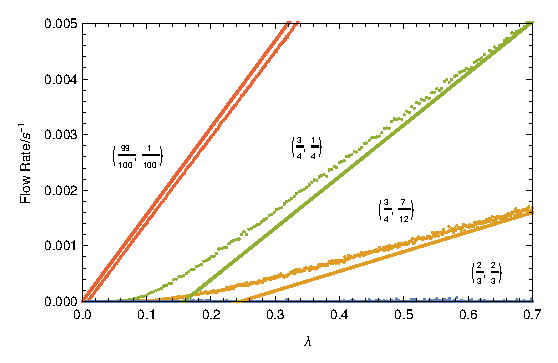
\includegraphics[width=0.5\linewidth]{../tex-src/lambdaScan/newFlowMean} & 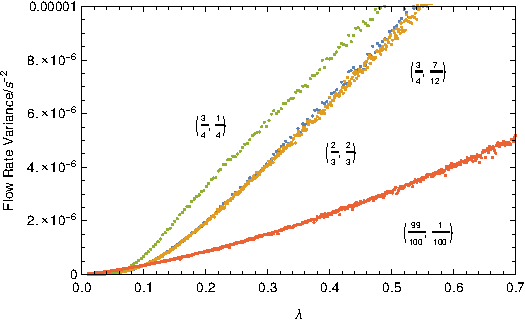
\includegraphics[width=0.5\linewidth]{../tex-src/lambdaScan/newFlowVar} \\
    \hline
    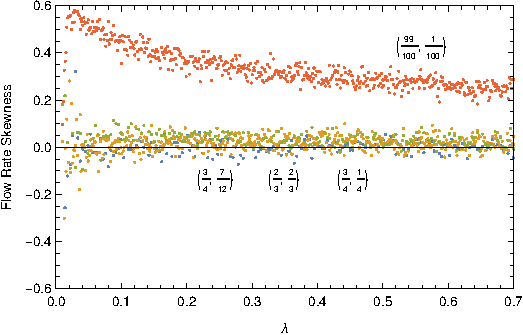
\includegraphics[width=0.5\linewidth]{../tex-src/lambdaScan/newFlowSkew} & 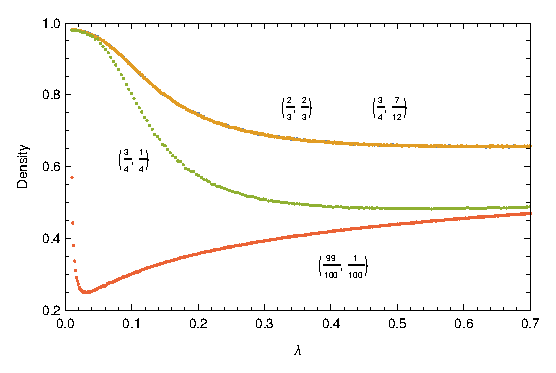
\includegraphics[width=0.5\linewidth]{../tex-src/lambdaScan/newDens} \\
    \end{tabular}
\end{center}
    \vspace{-0em}
\end{figure*}
\fi


The inset in Fig.~\ref{fig:lambdaScans} shows flow rates for
a range of $\lambda$ with four sets of boundary conditions.  
whilst the main body shows a log-log plot with a single set
of boundary conditions over a large range of $\lambda$.  
The equivalent MFT results are shown as a function of
$\lambda$ and $\delta\rho$, since the density within the system
$\rho(x)$, obtained by solving the cubic Eq. \ref{cubic}, is
non-unique for $\lambda<\frac{1}{4}$.  
The inset suggests that the SPM flow goes to zero, albeit at lower 
 $\lambda$ than implied by MFT.  However the main figure shows that some flow does 
continue, at a much reduced rate and with different power-law behavior from particle 
diffusion.  This different flow behavior defines the SPM transition.
For low-stickiness ($\lambda>\frac{1}{4}$) the MFT is in very good agreement with the
simulations, and this continues for repulsive $\lambda>>1$, where the
mean flow rate varies linearly with $\lambda$.


For very high-stickiness $\lambda<0.04$, convergence is very slow, hence
the large standard errors. However, there is a regime when $0.04 \le
\lambda \le 0.1$ where the mean flow displays clear $\mathcal{O}~(\lambda^{4})$ power-law behaviour.  The SPM
transition is where the power laws cross at $\lambda =
0.194$, in good agreement with the MFT switching to negative flow.
The key point here is that as that as we pass from high-$\lambda$ to
low-$\lambda$, the scaling in $\lambda$ does change, which suggests to
us that the mechanism by which material is transferred through the
medium changes from the standard diffusive one (which is
well-described by the MFT) to something different, which to our
knowledge has not been previously observed.
%However, one of the key predictions of the MFT - that a sharp transition to a no-flow regime occurs when $\lambda$ becomes small enough (at least for 3 of the 4 sets of
%boundary conditions we investigated here) - is not realized in our simulations. Indeed what seems to be happening is that the sharp transition has been smoothed out, as we
%do not see any peaks or jumps in the flow rate variance or skewness (which we would expect to see if there was a transition). We suspect that this discrepancy is due to nontrivial correlations emerging between the particles, which the MFT
%does not take account of. Alternatively, it could be that the continuum assumption is failing due to the finite-sized system filling with particles and blocking.

We also investigate varying both the driving force ($\delta\rho$) and
stickiness ($\lambda$), using boundaries $(\rho_0, \rho_L) = (\rho_M +
\frac{1}{2} \delta\rho, \rho_M - \frac{1}{2} \delta\rho)$ for some
given $\rho_M$. As before, we calculated flow rate moments and average
densities (Fig.~\ref{fig:constDens}).  The MFT prediction for the mean
flow is again a good fit until $\lambda$ becomes sufficiently small,
and as before the simulations show no evidence of negative diffusion;
rather the flow becomes critically slow for these very sticky
particles.  The higher moments of the flow (e.g. variance) do not show
sharp peaks, again indicating that the transition is a crossover in behaviour.  
The density within the system is very close to $\rho_M$ 
until $\lambda$ drops below 1/4, at which point the system fills $(\rho~\sim~1)$.
\begin{figure}[h!]
\vspace{1em}
\caption{\label{fig:constDens} Flow rate mean observed when varying the difference $\delta\rho$ between the boundary concentrations
$(\rho_0, \rho_L) = (\rho_M + \frac{1}{2} \delta\rho, \rho_M - \frac{1}{2} \delta\rho)$ and $\lambda$ (The top panel is the MFT prediction
for the flow rate, whilst bottom shows the observed mean flow rate).
We chose $\rho_M=\frac{1}{2}$, as this gives us the biggest range of $\delta\rho$ to investigate.
These calculations were performed with the same run parameters (system length etc)
as above.}
\begin{center}
 \begin{tabular}{c}
    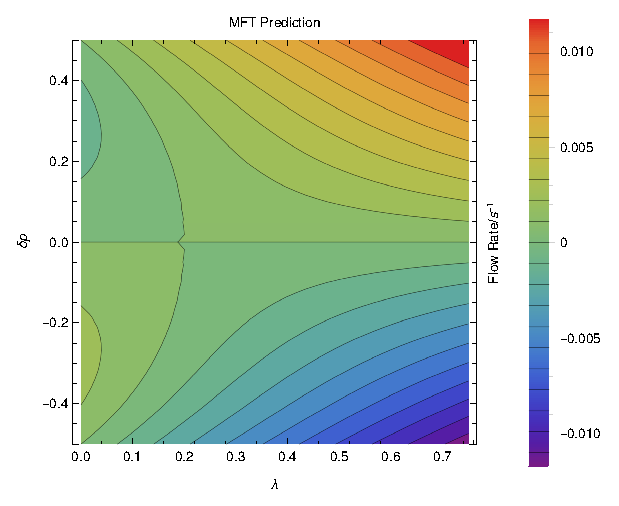
\includegraphics[width=0.98\linewidth]{newMftPred} \\
    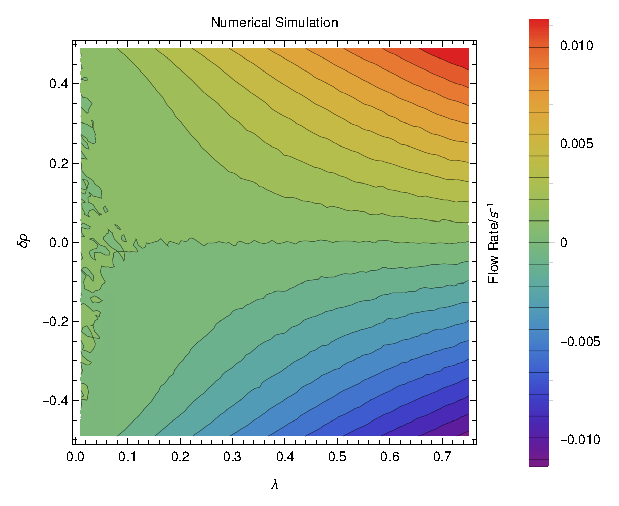
\includegraphics[width=0.98\linewidth]{newFlow}
    \end{tabular}
\end{center}
    \vspace{-2.5em}
\end{figure}


For relatively small driving force $\delta\rho$, we find
 $J$ varies approximately
linearly with $\delta\rho$, thus we can define 
$D_\mathrm{Eff}=\partDeriv{J}{\delta\rho}\big|_{\delta\rho=0}$, the effective diffusion coefficient and measure it using linear regression.
\begin{figure}[h!]
\vspace{1em}
\caption{\label{fig:diffCoef} Comparison of effective diffusion
  coefficient $D$ in the MFT (top) and in direct simulation (bottom)
  as a function of density and stickiness.  The region where MFT gives
  negative diffusion is represented as $D=0$. The simulations used 124
  sites averaged over $\sim 10^9$ steps at each of $12 \times 24
  \times 16 $ $(\lambda, \rho_M, \delta \rho)$ combinations.  Full
  details in the supplementary materials.}

\begin{center}
 \begin{tabular}{c}
    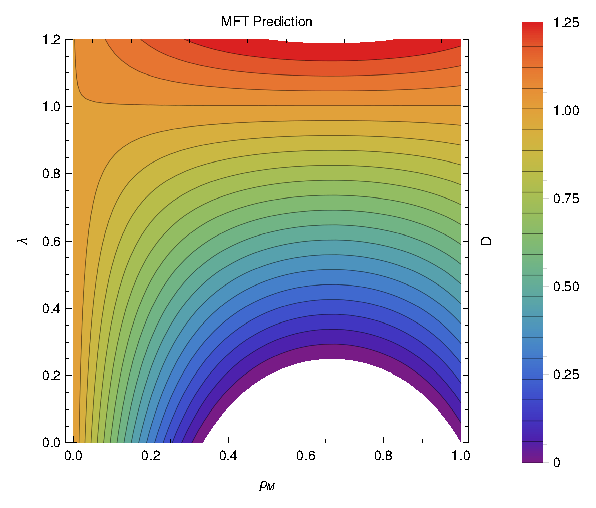
\includegraphics[width=0.98\linewidth]{newAnalFlow} \\
    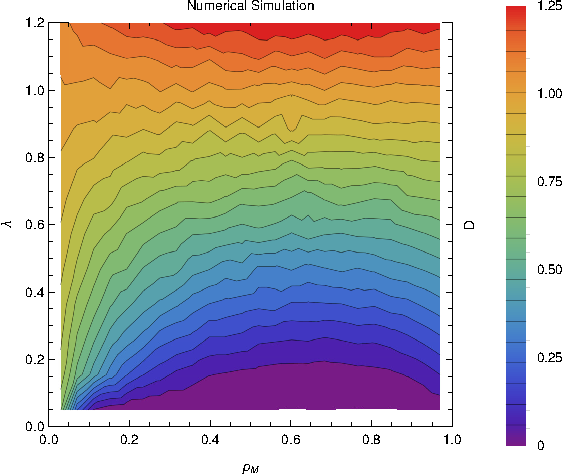
\includegraphics[width=0.98\linewidth]{newDataFlow}
    \end{tabular}
\end{center}
    \vspace{-2em}
\end{figure}

We compare the measured diffusion from (Fig.~\ref{fig:diffCoef}) with the MFT result (Eq.~\ref{eq:MFTflow})
The MFT
and simulation agree well for low stickiness, and both show the 
maximum $D$ at $\rho_M = \frac{2}{3}$. For high stickiness, where the
MFT prediction gives negative diffusion constant, measurement gives 
very low positive values for the current making determination of D difficult, however 
the important thing to note is that this critically slow flow corresponds to the
the negative - D region predicted by the MFT (indicated in purple).

It is instructive to get an overview of how the SPM particles move
during flow. Fig.~\ref{fig:flowPatterns} shows a plot of the flow
structure in an interesting regime.  Over short timescales little
structure is visible, the dynamics appearing as a random walk with
some tendency for particles to clump; over longer timescales the
diffusive behavior is more evident, with a textured structure
suggesting characteristic velocity of particles or vacancies through
emergent correlated clumps.  In the limiting case of low $\lambda$ the
density of particles in the system tends to 1, irrespective of
boundary density: this may be because the interactions between
particles are strong enough that the filled state has lower chemical 
potential than either boundary.  Another interesting case is the limit of
high $\lambda$, where irrespective of boundary density, the internal
density tends to $\rho=\frac{2}{3}$, the value which gives maximal
flow.  Additional plots can be found in the supplementary materials.

\begin{figure}[h!]
\caption{\label{fig:flowPatterns} Indicative spacetime flow pattern for sticky free-flow $\left[\lambda = \frac{3}{20}, (\rho_0, \rho_L) = (\frac{3}{4}, \frac{1}{4})\right]$; other combinations shown in the supplementary materials.
Time runs along the x-axis, space (1 pixel=1 site) along the y-axis, with grayscale tone (black being empty, white being full) illustrating average site occupation over (clockwise from top left) $\frac{1}{32}$, $1$, $8$ and $32$ Gillespie steps per site respectively.}
\begin{center}
 \begin{tabular}{c | c}
    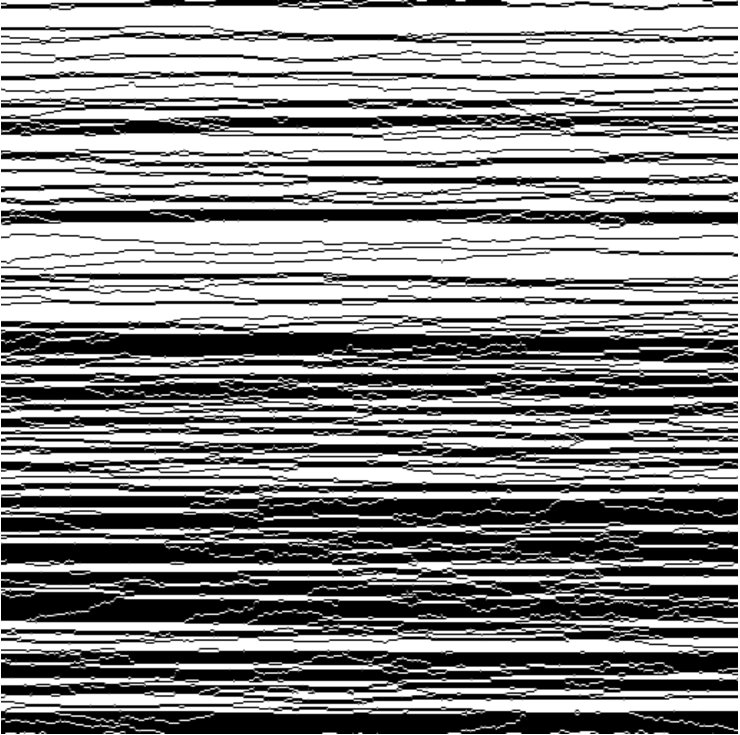
\includegraphics[width=0.49\linewidth]{shortTime}  &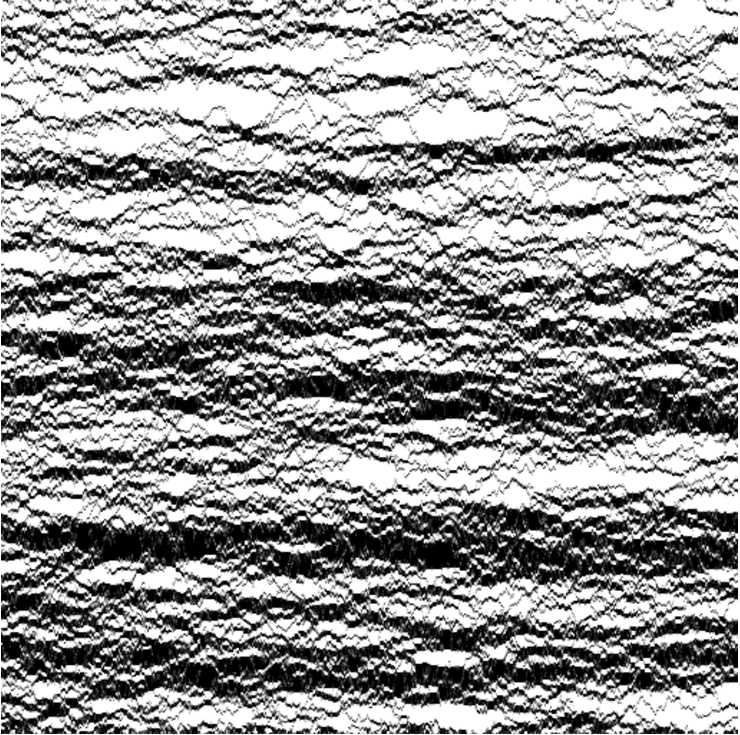
\includegraphics[width=0.49\linewidth]{midShortTime} \\
    \hline
    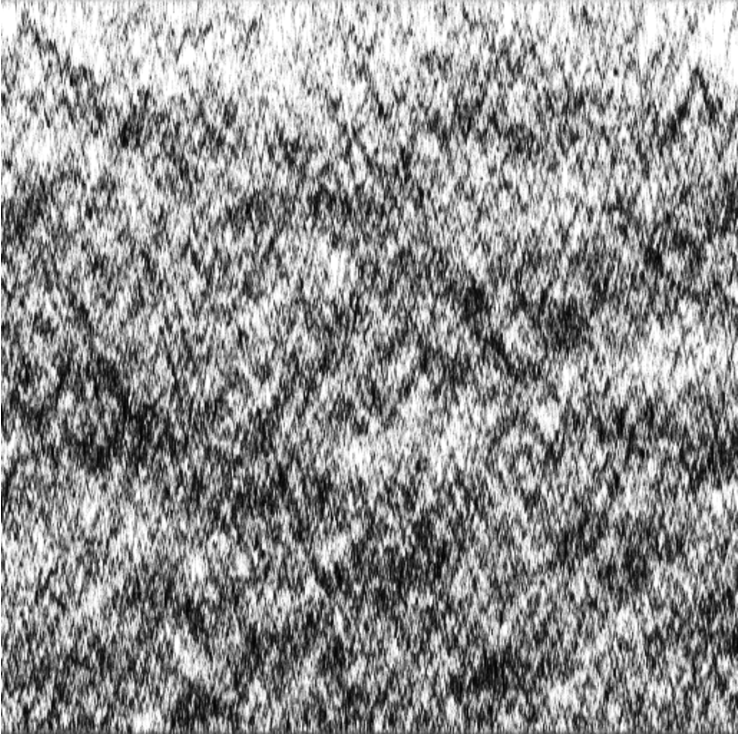
\includegraphics[width=0.49\linewidth]{longTime} &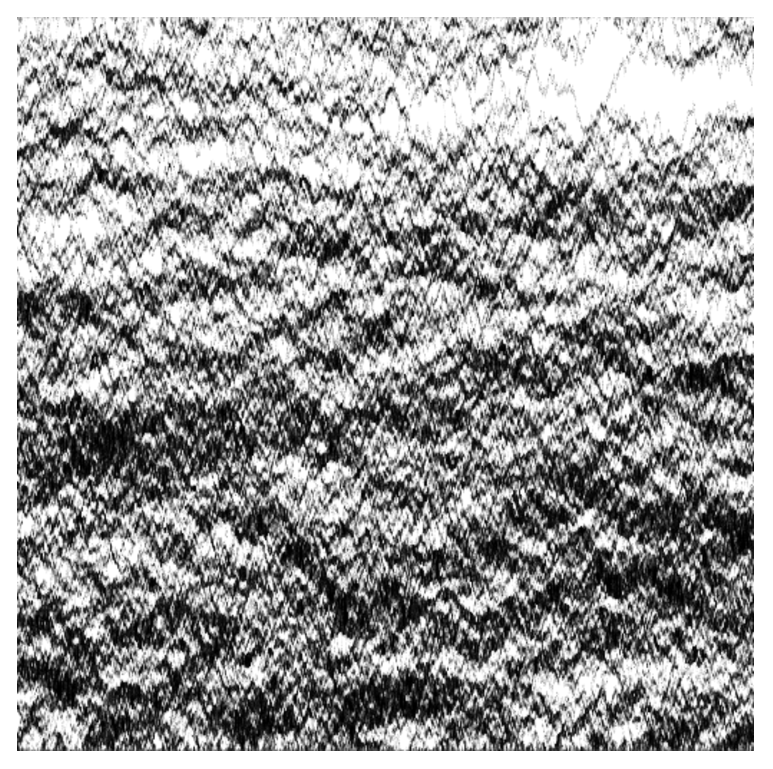
\includegraphics[width=0.49\linewidth]{midLongTime}
    \end{tabular}
\end{center}
    \vspace{-2em}
\end{figure}


To conclude, we have solved a nonlinear model for self-interacting sticky particles diffusing in 1D.  Although only the particles exhibit stickiness,  the analytics suggest a symmetry between vacancy-type and particle-type flow
at density of $\frac{2}{3}$, which is observed in the simulation.  The flow exhibits a foamy pattern with intermediate time-and-space correlations.  The continuum solution MFT is a good predictor of the bulk flow behavior of the SPM.
The negative diffusion constant found in MFT at high stickiness indicates  that the assumption of homogeneous density break down: thus the MFT predicts its own demise, and this agrees well with our numerics.

We would like to thank EPSRC (student grant 1527137) and Wolfson Foundation for providing the funding, Mikael Leetmaa for producing \texttt{KMCLib}, and the \texttt{Eddie3} team here at Edinburgh for maintaining the hardware used.
We would also like to thank Martin Evans, Bartek Waclaw and Richard Blythe for some very helpful discussions during the production of this letter.

\bibliography{jHellStickyParticleMain.bib}

\newpage


\end{document}
%
% ****** End of file apssamp.tex ******
